\documentclass[a4paper]{article}
\usepackage[margin = 1 in]{geometry}
\usepackage{fancyhdr}
\usepackage{lastpage}
\usepackage{ctex}
\usepackage[utf8]{inputenc} % Required for inputting international characters
\usepackage[T1]{fontenc} % Output font encoding for international characters
\usepackage[sfdefault]{ClearSans} % Use the Clear Sans font (sans serif)
\usepackage{tocloft} 
\usepackage[hidelinks]{hyperref}
\usepackage{makecell}%导入表格宏包
\usepackage{bmpsize}
\usepackage{graphicx}
\usepackage{epstopdf}
\usepackage{caption}
\usepackage{enumitem}
\usepackage{float}
\usepackage{multirow}
\usepackage{makecell}
\usepackage{amsmath} 
\usepackage{listings}
\usepackage{xcolor}

\author{Vergil/Zijun Li李子骏}
\title{Week 2}
\date{2023.4.10}

\lstset{
  language=Python,
  basicstyle=\ttfamily\small,
  numbers=left,
  numberstyle=\tiny\color{gray},
  stepnumber=1,
  numbersep=5pt,
  backgroundcolor=\color{white},
  showspaces=false,
  showstringspaces=false,
  showtabs=false,
  frame=single,
  rulecolor=\color{black},
  tabsize=4,
  captionpos=b,
  breaklines=true,
  breakatwhitespace=false,
  keywordstyle=\color{blue},
  commentstyle=\color{gray},
  stringstyle=\color{red}
}

\begin{document}
\maketitle
\noindent目前为了评估广告效果,希望基于广告曝光数据进行分析(广告曝光用户数据集):

\noindent1.	在全量数据及(data\_all.csv)中找到与广告曝光用户相似的用户,并看用户在不同特征上的分布差异?

\begin{figure}[H]
    \centering
    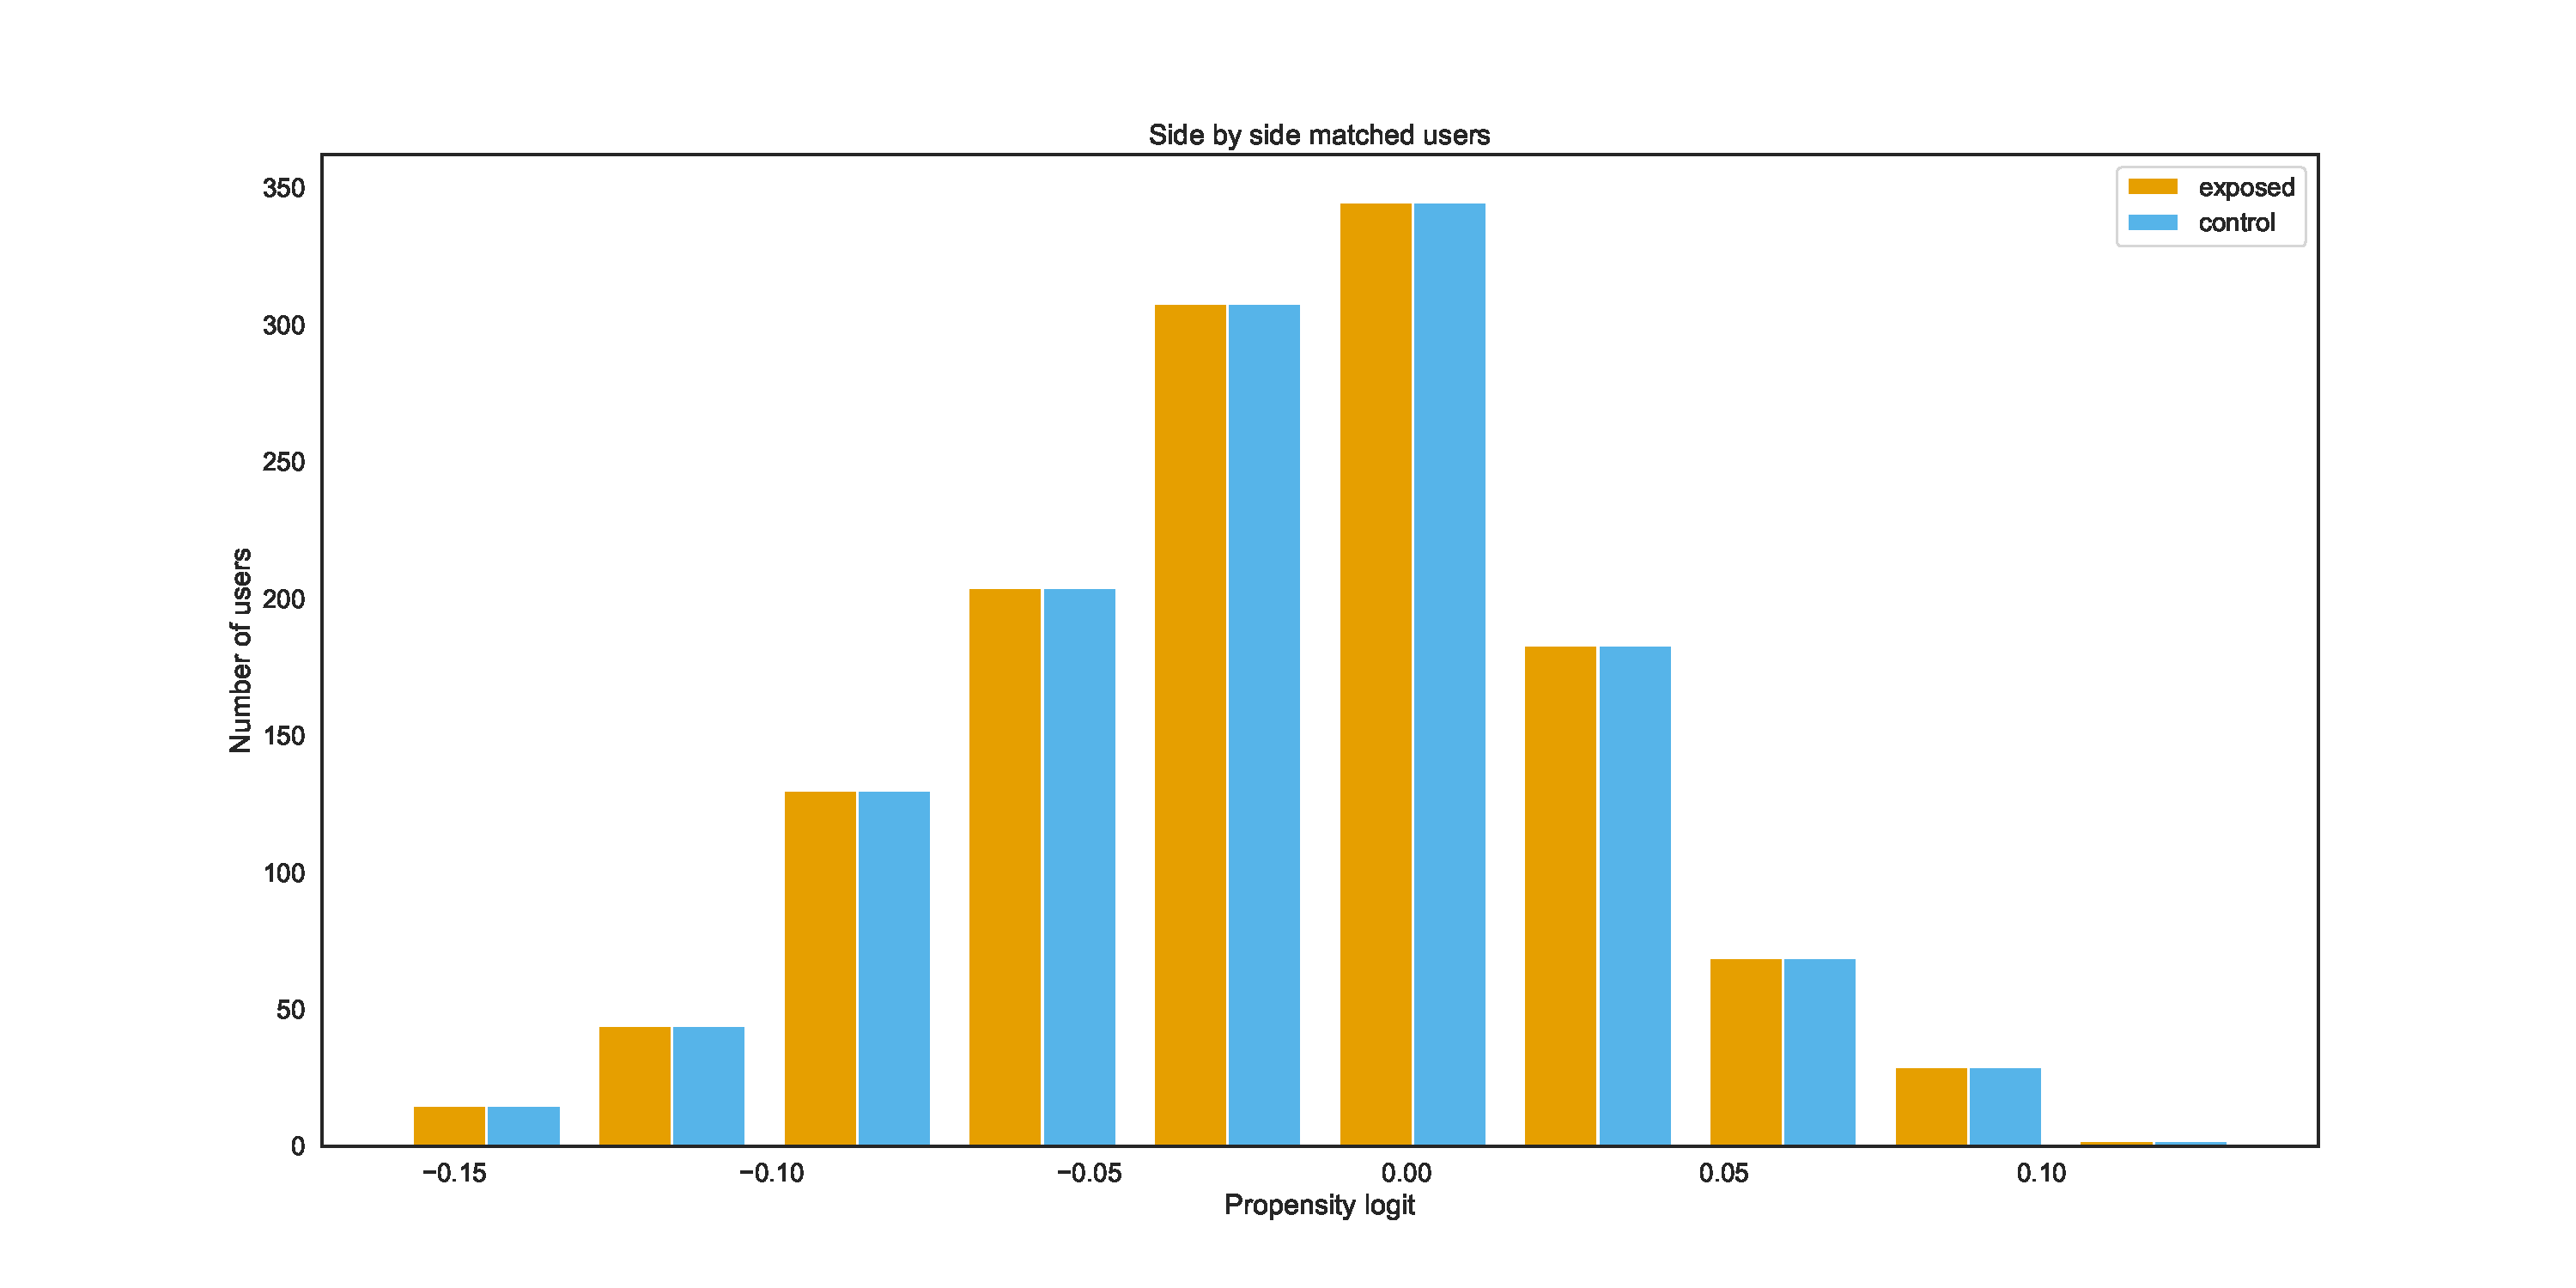
\includegraphics[width=1\textwidth]{./Side by side matched users.pdf}
    \label{fig:experiment1}
\end{figure}

这个图表显示了处理组(广告曝光用户)和对照组(未曝光用户)在倾向性评分上的分布. 从图上看, 两组的用户倾向性评分平衡. 匹配结果很好

\begin{figure}[H]
    \centering
    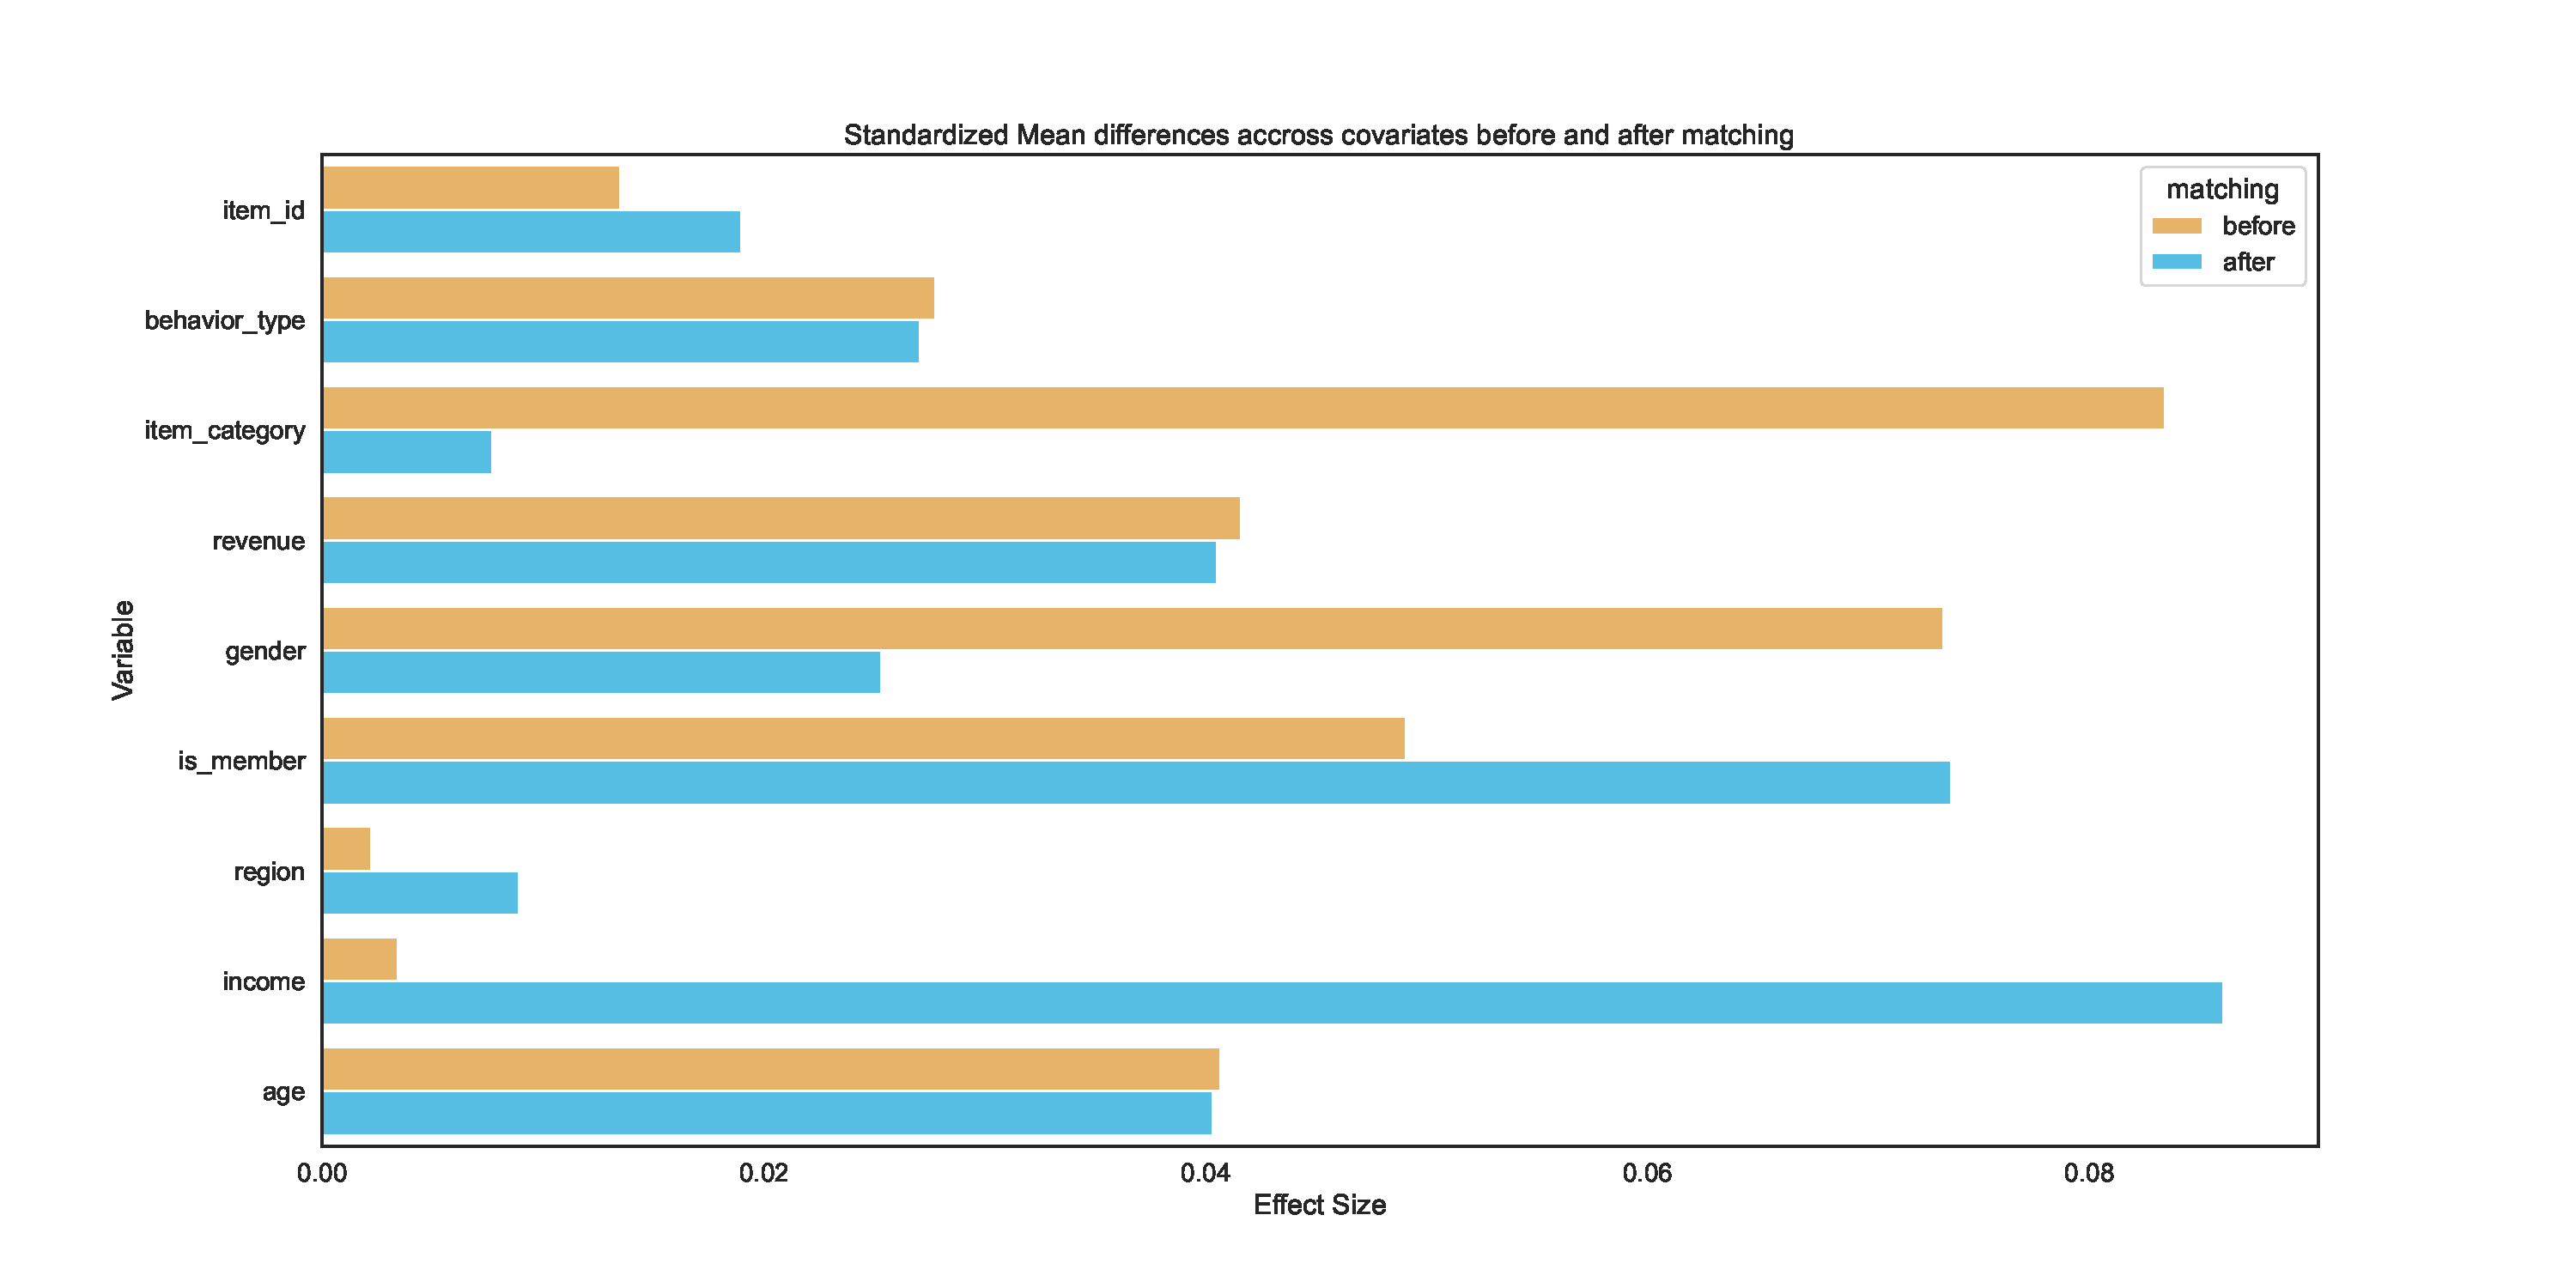
\includegraphics[width=1\textwidth]{./Standardized Mean differences accross covariates before an after matching.pdf}
    \label{fig:experiment2}
\end{figure}

这个图表显示了在匹配前后,处理组和对照组在各个特征上的标准化均值差异. 

\begin{itemize}
    \item 相同/类似: 行为, 购买金额, 年龄
    \item 不同: 物品类别, 性别, 会员, 地区, 收入
\end{itemize}

\noindent2.	广告曝光用户人均消费是否高于未被广告曝光且相似用户?在哪个行为类型(behavior\_type)的专户上更高?

\begin{lstlisting}[language=Python]
    exposed_matched = psm.df_matched[psm.df_matched['exposed'] == 1]
    non_exposed_matched = psm.df_matched[psm.df_matched['exposed'] == 0]
    
    consumption_diff = exposed_matched.groupby('behavior_type')['revenue'].mean() - non_exposed_matched.groupby('behavior_type')['revenue'].mean()
    print(consumption_diff)

    # 55.351813
\end{lstlisting}

标准差为55.35(基于全组), 明显高于


\begin{lstlisting}[language=Python]
    behavior_types = [1, 2, 3]

    for b_type in behavior_types:
        exposed_matched_filtered = exposed_matched[exposed_matched['behavior_type'] == b_type]
        non_exposed_matched_filtered = non_exposed_matched[non_exposed_matched['behavior_type'] == b_type]

        exposed_purchase = exposed_matched[exposed_matched['behavior_type'] == 4]
        non_exposed_purchase = non_exposed_matched[non_exposed_matched['behavior_type'] == 4]

        exposed_conversion_rate = len(exposed_purchase) / len(exposed_matched_filtered)
        print(f"exposed_conversion_rate for behavior type {b_type}: {exposed_conversion_rate}")
        non_exposed_conversion_rate = len(non_exposed_purchase) / len(non_exposed_matched_filtered)
        print(f"non_exposed_conversion_rate for behavior type {b_type}: {non_exposed_conversion_rate}")

        conversion_rate_diff = exposed_conversion_rate - non_exposed_conversion_rate
        print(f"Conversion rate difference for behavior type {b_type}: {conversion_rate_diff}")

    # exposed_conversion_rate for behavior type 1: 0.01607717041800643
    # non_exposed_conversion_rate for behavior type 1: 0.019077901430842606
    # Conversion rate difference for behavior type 1: -0.003000731012836176
    # exposed_conversion_rate for behavior type 2: 0.7407407407407407
    # non_exposed_conversion_rate for behavior type 2: 1.1428571428571428
    # Conversion rate difference for behavior type 2: -0.4021164021164021
    # exposed_conversion_rate for behavior type 3: 0.5263157894736842
    # non_exposed_conversion_rate for behavior type 3: 0.9230769230769231
    # Conversion rate difference for behavior type 3: -0.39676113360323895
\end{lstlisting}

Conversion rate difference for behavior type 1: -0.003000731012836176

Conversion rate difference for behavior type 2: -0.4021164021164021

Conversion rate difference for behavior type 3: -0.39676113360323895

广告曝光用户的购买转化率都低于未被广告曝光的相似用户

可能对转化率产生了负面影响

相比较而言, 收藏的购买转化率差异最大,其次是加购物车

\end{document}